\section{Model matematyczny obiektu TRAS}

\begin{figure}[!htb]
  \centering
  \begin{subfigure}[b]{0.4\textwidth}
    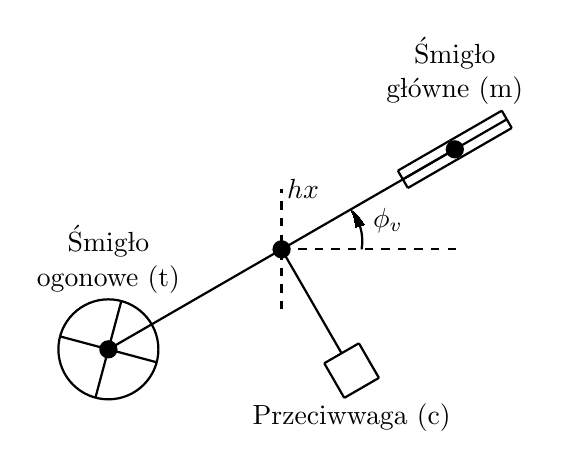
\begin{tikzpicture}[scale=2.54]
% dpic version 2015.10.28 option -g for TikZ and PGF 1.01
\ifx\dpiclw\undefined\newdimen\dpiclw\fi
\global\def\dpicdraw{\draw[line width=\dpiclw]}
\global\def\dpicstop{;}
\dpiclw=0.8bp
\dpicdraw (0.25,0) circle (0.098425in)\dpicstop
\dpicdraw (0.314714,0.241479)
 --(0.185264,-0.241473)\dpicstop
\dpicdraw (0.491482,-0.064703)
 --(0.008512,0.064681)\dpicstop
\dpicdraw[fill=black](0.25,0) circle (0.015748in)\dpicstop
\dpicdraw (0.25,0)
 --(1.116033,0.499987)\dpicstop
\dpicdraw[fill=black](1.116033,0.499987) circle (0.015748in)\dpicstop
\dpicdraw (1.116033,0.499987)
 --(1.982066,0.999973)\dpicstop
\dpicdraw (1.722266,0.849975)
 --(1.747268,0.806674)\dpicstop
\dpicdraw (1.747268,0.806674)
 --(2.007077,0.95667)\dpicstop
\dpicdraw (2.007077,0.95667)
 --(2.266887,1.106666)\dpicstop
\dpicdraw (2.266887,1.106666)
 --(2.24189,1.149969)\dpicstop
\dpicdraw (2.24189,1.149969)
 --(2.216893,1.193272)\dpicstop
\dpicdraw (2.216893,1.193272)
 --(1.957069,1.0433)\dpicstop
\dpicdraw (1.957069,1.0433)
 --(1.697245,0.893328)\dpicstop
\dpicdraw (1.697245,0.893328)
 --(1.722246,0.850028)\dpicstop
\dpicdraw[fill=black](1.982073,0.999985) circle (0.015748in)\dpicstop
\dpicdraw (1.722266,0.849975)
 --(2.24189,1.149969)\dpicstop
\dpicdraw (1.379445,-0.156224)
 --(1.429448,-0.242825)\dpicstop
\dpicdraw (1.429448,-0.242825)
 --(1.516051,-0.192826)\dpicstop
\dpicdraw (1.516051,-0.192826)
 --(1.602654,-0.142827)\dpicstop
\dpicdraw (1.602654,-0.142827)
 --(1.55266,-0.056222)\dpicstop
\dpicdraw (1.55266,-0.056222)
 --(1.502665,0.030384)\dpicstop
\dpicdraw (1.502665,0.030384)
 --(1.416057,-0.019607)\dpicstop
\dpicdraw (1.416057,-0.019607)
 --(1.329449,-0.069597)\dpicstop
\dpicdraw (1.329449,-0.069597)
 --(1.379452,-0.156198)\dpicstop
\dpicdraw (1.416057,-0.019607)
 --(1.116033,0.499987)\dpicstop
\dpicdraw[dashed](1.116033,0.499987)
 --(2.016033,0.499987)\dpicstop
\filldraw[line width=0bp](1.508303,0.616532)
 --(1.486091,0.609517)
 ..controls (1.483969,0.640891) and (1.475947,0.671582)
 ..(1.462446,0.699981)
 ..controls (1.490164,0.67947) and (1.513339,0.653447)
 ..(1.530514,0.623548)
 --(1.508303,0.616532)\dpicstop
\dpicdraw[line width=0.8bp](1.488044,0.662374)
 ..controls (1.515457,0.612963) and (1.525323,0.555723)
 ..(1.516033,0.499987)\dpicstop
\draw (1.647293,0.642333) node{$\phi_v$};
\draw (0.25,0.45) node{\shortstack{Śmigło\\%
ogonowe (t)}};
\draw (1.982066,1.393272) node{\shortstack{Śmigło\\%
główne (m)}};
\draw (1.466052,-0.242825) node[below=-1.5bp]{Przeciwwaga (c)};
\dpicdraw[dashed](1.116033,0.199987)
 --(1.116033,0.799987)\dpicstop
\draw (1.116033,0.799987) node[right=-1.5bp]{$hx$};
\end{tikzpicture}

    \caption{Urządzenie (widok z boku)}
    \label{rys:schtrasv}
  \end{subfigure}
  \begin{subfigure}[b]{0.25\textwidth}
    \input{img/pic_tras_model_schematic_v.tex}
    \vspace{0.8cm}
    \caption{Model}
    \label{rys:schmodelv}
  \end{subfigure}
  \caption{Schemat systemu TRAS w płaszczyźnie pionowej}
\end{figure}

\begin{figure}[!htb]
  \centering
  \begin{subfigure}[b]{0.4\textwidth}
    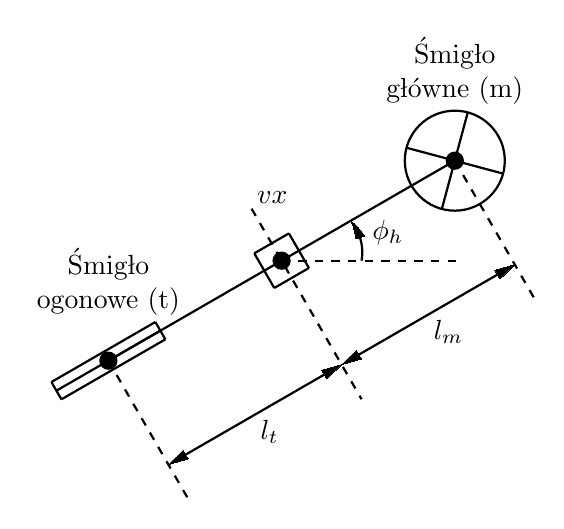
\begin{tikzpicture}[scale=2.54]
% dpic version 2015.10.28 option -g for TikZ and PGF 1.01
\ifx\dpiclw\undefined\newdimen\dpiclw\fi
\global\def\dpicdraw{\draw[line width=\dpiclw]}
\global\def\dpicstop{;}
\dpiclw=0.8bp
\dpicdraw (0.025021,-0.149998)
 --(0.050022,-0.193299)\dpicstop
\dpicdraw (0.050022,-0.193299)
 --(0.309832,-0.043303)\dpicstop
\dpicdraw (0.309832,-0.043303)
 --(0.569642,0.106693)\dpicstop
\dpicdraw (0.569642,0.106693)
 --(0.544645,0.149996)\dpicstop
\dpicdraw (0.544645,0.149996)
 --(0.519648,0.193299)\dpicstop
\dpicdraw (0.519648,0.193299)
 --(0.259824,0.043327)\dpicstop
\dpicdraw (0.259824,0.043327)
 --(0,-0.106645)\dpicstop
\dpicdraw (0,-0.106645)
 --(0.025001,-0.149946)\dpicstop
\dpicdraw[fill=black](0.284828,0.000012) circle (0.015748in)\dpicstop
\dpicdraw (0.025021,-0.149998)
 --(0.544645,0.149996)\dpicstop
\dpicdraw (0.284821,0)
 --(1.150854,0.499987)\dpicstop
\dpicdraw[fill=black](1.150854,0.499987) circle (0.015748in)\dpicstop
\dpicdraw (1.150854,0.499987)
 --(2.016887,0.999973)\dpicstop
\dpicdraw (2.016887,0.999973) circle (0.098425in)\dpicstop
\dpicdraw (2.081601,1.241452)
 --(1.952151,0.7585)\dpicstop
\dpicdraw (2.258369,0.93527)
 --(1.775399,1.064654)\dpicstop
\dpicdraw[fill=black](2.016887,0.999973) circle (0.015748in)\dpicstop
\dpicdraw[dashed](1.150854,0.499987)
 --(2.050854,0.499987)\dpicstop
\filldraw[line width=0bp](1.543124,0.616532)
 --(1.520912,0.609517)
 ..controls (1.51879,0.640891) and (1.510768,0.671582)
 ..(1.497268,0.699981)
 ..controls (1.524985,0.67947) and (1.54816,0.653447)
 ..(1.565335,0.623548)
 --(1.543124,0.616532)\dpicstop
\dpicdraw[line width=0.8bp](1.522866,0.662374)
 ..controls (1.550279,0.612963) and (1.560144,0.555723)
 ..(1.550854,0.499987)\dpicstop
\draw (1.682115,0.642333) node{$\phi_h$};
\dpicdraw (1.064248,0.449983)
 --(1.11425,0.363382)\dpicstop
\dpicdraw (1.11425,0.363382)
 --(1.200854,0.413381)\dpicstop
\dpicdraw (1.200854,0.413381)
 --(1.287457,0.46338)\dpicstop
\dpicdraw (1.287457,0.46338)
 --(1.237462,0.549985)\dpicstop
\dpicdraw (1.237462,0.549985)
 --(1.187468,0.636591)\dpicstop
\dpicdraw (1.187468,0.636591)
 --(1.10086,0.5866)\dpicstop
\dpicdraw (1.10086,0.5866)
 --(1.014252,0.53661)\dpicstop
\dpicdraw (1.014252,0.53661)
 --(1.064254,0.450009)\dpicstop
\draw (0.284821,0.393299) node{\shortstack{Śmigło\\%
ogonowe (t)}};
\draw (2.016887,1.449973) node{\shortstack{Śmigło\\%
główne (m)}};
\dpicdraw[dashed](1.00087,0.759804)
 --(1.550876,-0.192821)\dpicstop
\dpicdraw[dashed](0.284821,0)
 --(0.684843,-0.692808)\dpicstop
\dpicdraw[dashed](2.016887,0.999973)
 --(2.416909,0.307165)\dpicstop
\draw (1.00087,0.759804) node[above right=-1.5bp]{$vx$};
\filldraw[line width=0bp](1.376767,-0.091269)
 --(1.45087,-0.019619)
 --(1.351767,-0.047967) --cycle\dpicstop
\filldraw[line width=0bp](0.658941,-0.447956)
 --(0.584837,-0.519606)
 --(0.68394,-0.491258) --cycle\dpicstop
\dpicdraw (1.431033,-0.031072)
 --(0.604675,-0.508153)\dpicstop
\draw (1.017854,-0.269613) node[below right=-1.5bp]{$l_t$};
\filldraw[line width=0bp](1.524974,0.05203)
 --(1.45087,-0.019619)
 --(1.549973,0.008728) --cycle\dpicstop
\filldraw[line width=0bp](2.2428,0.408718)
 --(2.316903,0.480367)
 --(2.2178,0.452019) --cycle\dpicstop
\dpicdraw (1.470708,-0.008167)
 --(2.297066,0.468915)\dpicstop
\draw (1.883887,0.230374) node[below right=-1.5bp]{$l_m$};
\end{tikzpicture}

    \caption{Urządzenie (widok z góry)}
    \label{rys:schtrash}
  \end{subfigure}
  \begin{subfigure}[b]{0.25\textwidth}
    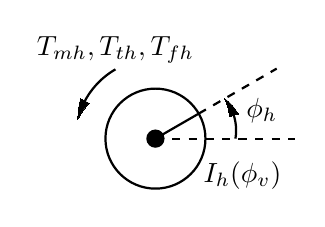
\begin{tikzpicture}[scale=2.54]
% dpic version 2015.10.28 option -g for TikZ and PGF 1.01
\ifx\dpiclw\undefined\newdimen\dpiclw\fi
\global\def\dpicdraw{\draw[line width=\dpiclw]}
\global\def\dpicstop{;}
\dpiclw=0.8bp
\dpicdraw (0.25,0) circle (0.098425in)\dpicstop
\draw (0.463388,-0.088388) node[below right=-1.5bp]{$I_h(\phi_v)$};
\dpicdraw[fill=black](0.25,0) circle (0.015748in)\dpicstop
\dpicdraw[dashed](0.25,0)
 --(0.95,0)\dpicstop
\dpicdraw (0.25,0)
 --(0.466508,0.124997)\dpicstop
\dpicdraw[dashed](0.466508,0.124997)
 --(0.856223,0.349991)\dpicstop
\filldraw[line width=0bp](0.642269,0.116546)
 --(0.620058,0.109531)
 ..controls (0.617936,0.140904) and (0.609914,0.171595)
 ..(0.596413,0.199995)
 ..controls (0.624131,0.179484) and (0.647306,0.15346)
 ..(0.664481,0.123561)
 --(0.642269,0.116546)\dpicstop
\dpicdraw[line width=0.8bp](0.622011,0.162387)
 ..controls (0.649424,0.112977) and (0.65929,0.055737)
 ..(0.65,0)\dpicstop
\draw (0.78126,0.142346) node{$\phi_h$};
\filldraw[line width=0bp](-0.103189,0.188492)
 --(-0.081983,0.177175)
 ..controls (-0.103746,0.153112) and (-0.122501,0.126492)
 ..(-0.137835,0.097899)
 ..controls (-0.137756,0.132306) and (-0.133239,0.166559)
 ..(-0.124394,0.199809)
 --(-0.103189,0.188492)\dpicstop
\dpicdraw[line width=0.8bp](-0.124183,0.141376)
 ..controls (-0.091534,0.22779) and (-0.029981,0.300239)
 ..(0.050021,0.346423)\dpicstop
\draw (0.050021,0.346423) node[above=-1.5bp]{$T_{mh},T_{th},T_{fh}$};
\end{tikzpicture}

    \vspace{2.7cm}
    \caption{Model}
    \label{rys:schmodelh}
  \end{subfigure}
  \caption{Schemat systemu TRAS w płaszczyźnie poziomej}
\end{figure}

\begin{figure}[!htb]
  \centering
  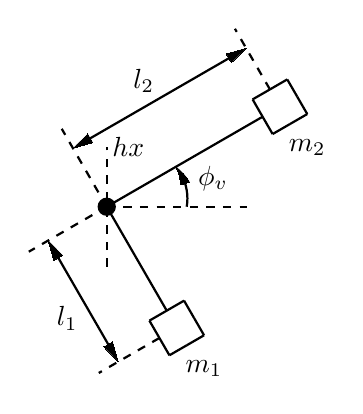
\begin{tikzpicture}[scale=2.54]
% dpic version 2015.10.28 option -g for TikZ and PGF 1.01
\ifx\dpiclw\undefined\newdimen\dpiclw\fi
\global\def\dpicdraw{\draw[line width=\dpiclw]}
\global\def\dpicstop{;}
\dpiclw=0.8bp
\dpicdraw[fill=black](0,0) circle (0.015748in)\dpicstop
\dpicdraw (0.779426,0.449983)
 --(0.829429,0.363382)\dpicstop
\dpicdraw (0.829429,0.363382)
 --(0.916032,0.413381)\dpicstop
\dpicdraw (0.916032,0.413381)
 --(1.002636,0.46338)\dpicstop
\dpicdraw (1.002636,0.46338)
 --(0.952641,0.549985)\dpicstop
\dpicdraw (0.952641,0.549985)
 --(0.902646,0.636591)\dpicstop
\dpicdraw (0.902646,0.636591)
 --(0.816038,0.5866)\dpicstop
\dpicdraw (0.816038,0.5866)
 --(0.729431,0.53661)\dpicstop
\dpicdraw (0.729431,0.53661)
 --(0.779433,0.450009)\dpicstop
\dpicdraw (0.779426,0.449983)
 --(0,0)\dpicstop
\draw (1.002636,0.363382) node[below=-1.5bp]{$m_2$};
\dpicdraw (0.263412,-0.65621)
 --(0.313415,-0.742811)\dpicstop
\dpicdraw (0.313415,-0.742811)
 --(0.400018,-0.692813)\dpicstop
\dpicdraw (0.400018,-0.692813)
 --(0.486621,-0.642814)\dpicstop
\dpicdraw (0.486621,-0.642814)
 --(0.436627,-0.556208)\dpicstop
\dpicdraw (0.436627,-0.556208)
 --(0.386632,-0.469603)\dpicstop
\dpicdraw (0.386632,-0.469603)
 --(0.300024,-0.519593)\dpicstop
\dpicdraw (0.300024,-0.519593)
 --(0.213416,-0.569584)\dpicstop
\dpicdraw (0.213416,-0.569584)
 --(0.263419,-0.656185)\dpicstop
\dpicdraw (0.300024,-0.519593)
 --(0,0)\dpicstop
\draw (0.486621,-0.742811) node[below=-1.5bp]{$m_1$};
\dpicdraw[dashed](0.816038,0.5866)
 --(0.641057,0.889712)\dpicstop
\dpicdraw[dashed](0,0)
 --(-0.224976,0.389725)\dpicstop
\filldraw[line width=0bp](0.623198,0.720631)
 --(0.697301,0.792281)
 --(0.598198,0.763933) --cycle\dpicstop
\filldraw[line width=0bp](-0.094628,0.363943)
 --(-0.168732,0.292294)
 --(-0.069629,0.320642) --cycle\dpicstop
\dpicdraw (0.677464,0.780828)
 --(-0.148894,0.303747)\dpicstop
\draw (0.264285,0.542287) node[above left=-1.5bp]{$l_2$};
\dpicdraw[dashed](0.263412,-0.65621)
 --(-0.039696,-0.831201)\dpicstop
\dpicdraw[dashed](0,0)
 --(-0.389715,-0.224994)\dpicstop
\filldraw[line width=0bp](-0.01392,-0.700852)
 --(0.057733,-0.774952)
 --(0.02938,-0.675851) --cycle\dpicstop
\filldraw[line width=0bp](-0.220633,-0.242846)
 --(-0.292286,-0.168745)
 --(-0.263934,-0.267847) --cycle\dpicstop
\dpicdraw (0.046279,-0.755116)
 --(-0.280832,-0.188582)\dpicstop
\draw (-0.117277,-0.471849) node[below left=-1.5bp]{$l_1$};
\dpicdraw[dashed](0,0)
 --(0.7,0)\dpicstop
\filldraw[line width=0bp](0.392269,0.116546)
 --(0.370058,0.109531)
 ..controls (0.367936,0.140904) and (0.359914,0.171595)
 ..(0.346413,0.199995)
 ..controls (0.374131,0.179484) and (0.397306,0.15346)
 ..(0.414481,0.123561)
 --(0.392269,0.116546)\dpicstop
\dpicdraw[line width=0.8bp](0.372011,0.162387)
 ..controls (0.399424,0.112977) and (0.40929,0.055737)
 ..(0.4,-0)\dpicstop
\draw (0.53126,0.142346) node{$\phi_v$};
\dpicdraw[dashed](0,-0.3)
 --(0,0.3)\dpicstop
\draw (0,0.3) node[right=-1.5bp]{$hx$};
\end{tikzpicture}

  \label{rys:schih}
  \caption{Model układu mas dla momentu bezwładności $I_h(\phi_v)$}
\end{figure}

\newpage

Momenty działające na helikopter w płaszczyźnie pionowej:

\begin{equation}
  \begin{cases}
    T_{mv} & = l_mF_m(\omega_m) \\
    T_{tv} & = a_{tv}\omega_t \\
    T_{fv} & = -f_v\dot{\phi}_v \\
    T_g    & = -l_rm_rg\sin(\phi_v-\phi_{v0}) \\
  \end{cases}
\end{equation}

Momenty działające na helikopter w płaszczyźnie poziomej:

\begin{equation}
  \begin{cases}
    T_{mh} & = a_{mh}\omega_m\cos\phi_v \\
    T_{th} & = l_tF_t(\omega_t)\cos\phi_v \\
    T_{fh} & = -f_h\dot{\phi}_h \\
  \end{cases}
\end{equation}

Równania dynamiki modelu:

\begin{equation}
  \begin{cases}
    \ddot{\phi}_vI_v         & = T_{mv} + T_{tv} + T_{fv} + T_g \\
    \ddot{\phi}_hI_h(\phi_v) & = T_{mh} + T_{th} + T_{fh} \\
  \end{cases}
\end{equation}

Równania dynamiki silników:

\begin{equation}
  \begin{cases}
    \dot{\omega}_ma_m & = u_m - H_m^{-1}(\omega_m) \\
    \dot{\omega}_ta_t & = u_t - H_t^{-1}(\omega_t) \\
  \end{cases}
\end{equation}

Dokonując pewnych przekształceń, dostajemy układ równań dynamiki kompletnego
systemu:

\begin{equation}
  \begin{cases}
    \dot{x}_1 & = x_2 \\
    \dot{x}_2I_v & = l_mF_m(x_5) + a_{tv}x_6 -
    f_vx_2 - l_rm_rg\sin(x_1-\phi_{v0}) \\
    \dot{x}_3 & = x_4 \\
    \dot{x}_4I_h(x_1) & = (a_{mh}x_5 +
    l_tF_t(x_6))\cos x_1 - f_hx_4 \\
    \dot{x}_5a_m & = u_m - H_m^{-1}(x_5) \\
    \dot{x}_6a_t & = u_t - H_t^{-1}(x_6) \\
  \end{cases}
\end{equation}

